\documentclass[12pt,a4paper]{article}
\usepackage[utf8]{ inputenc }
\usepackage[russian]{ babel }
\usepackage[left=2.0cm, top=1.5cm, right=2.0cm, bottom=2.5cm]{ geometry }
\usepackage{ indentfirst }
\sloppy
\usepackage{ amsmath }
\usepackage{ amsfonts }
\usepackage{ amssymb }
\usepackage{ graphicx }
\usepackage{ subfig }
\usepackage{ gensymb }
\usepackage{ multicol } 
\newcommand{\numofcol}{6}
\graphicspath{{images/}}

\begin{document}

\section{Выбор площадок}
	\begin{figure}[h!]
		\begin{center}
		\begin{tabular}{c}
			\subfloat[30 MHz]{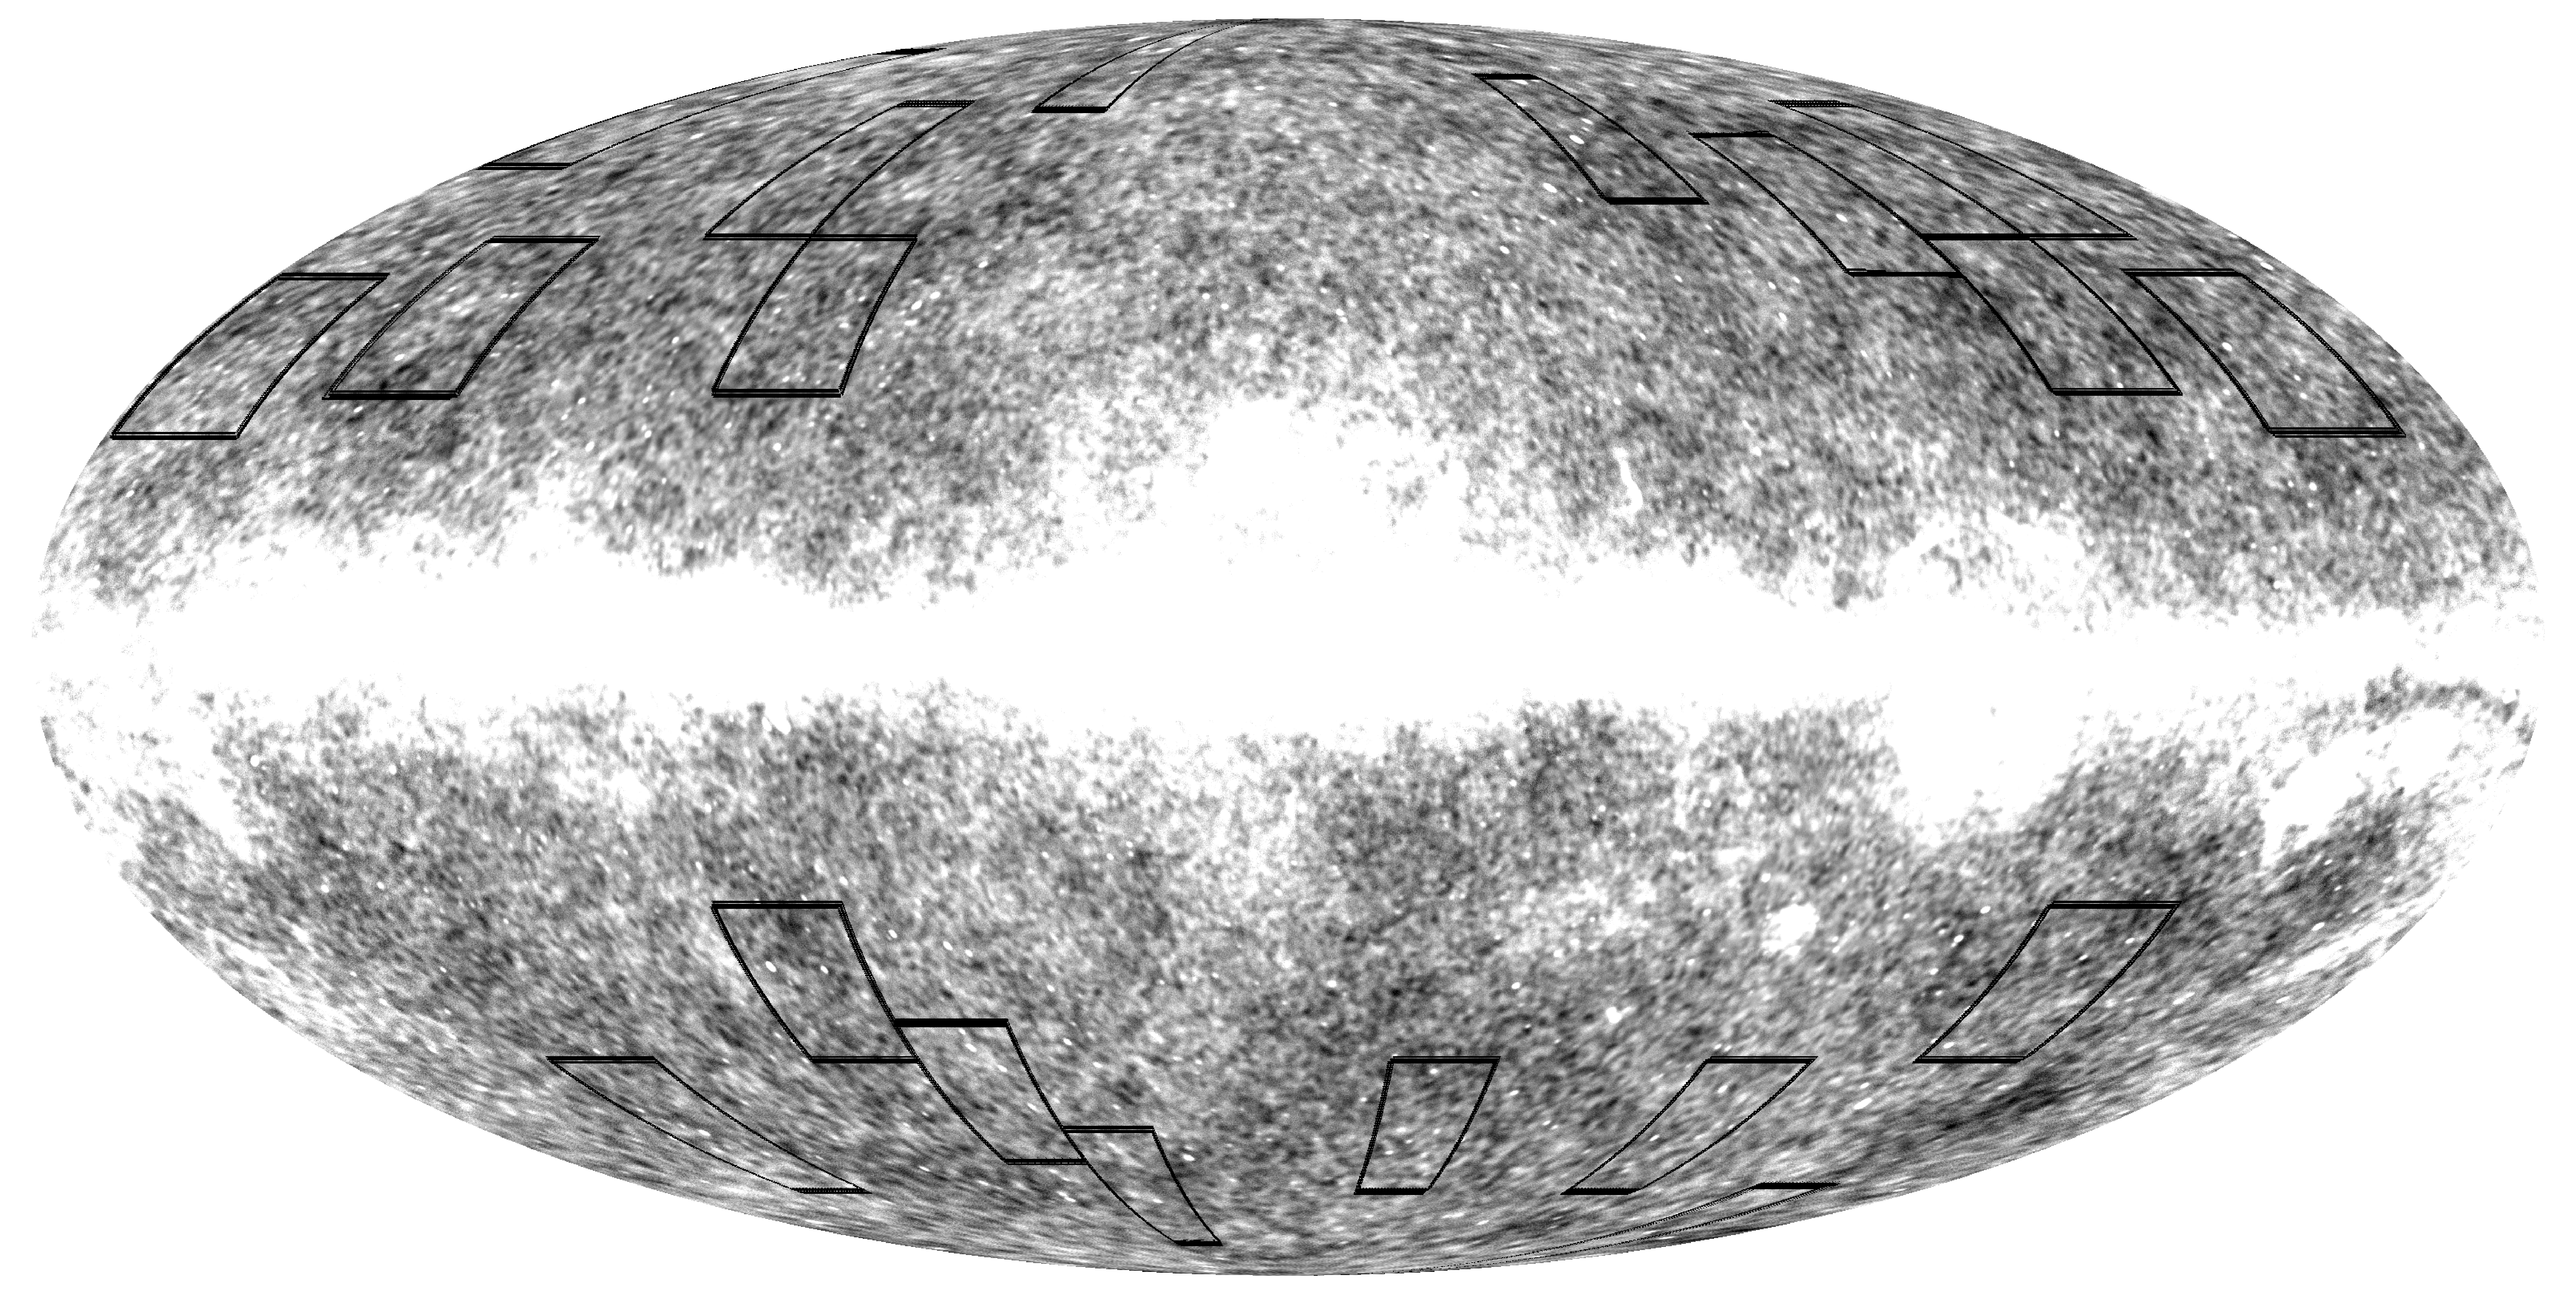
\includegraphics[width=0.9\textwidth]{areas_030_wb}} \\
			\subfloat[217 MHz]{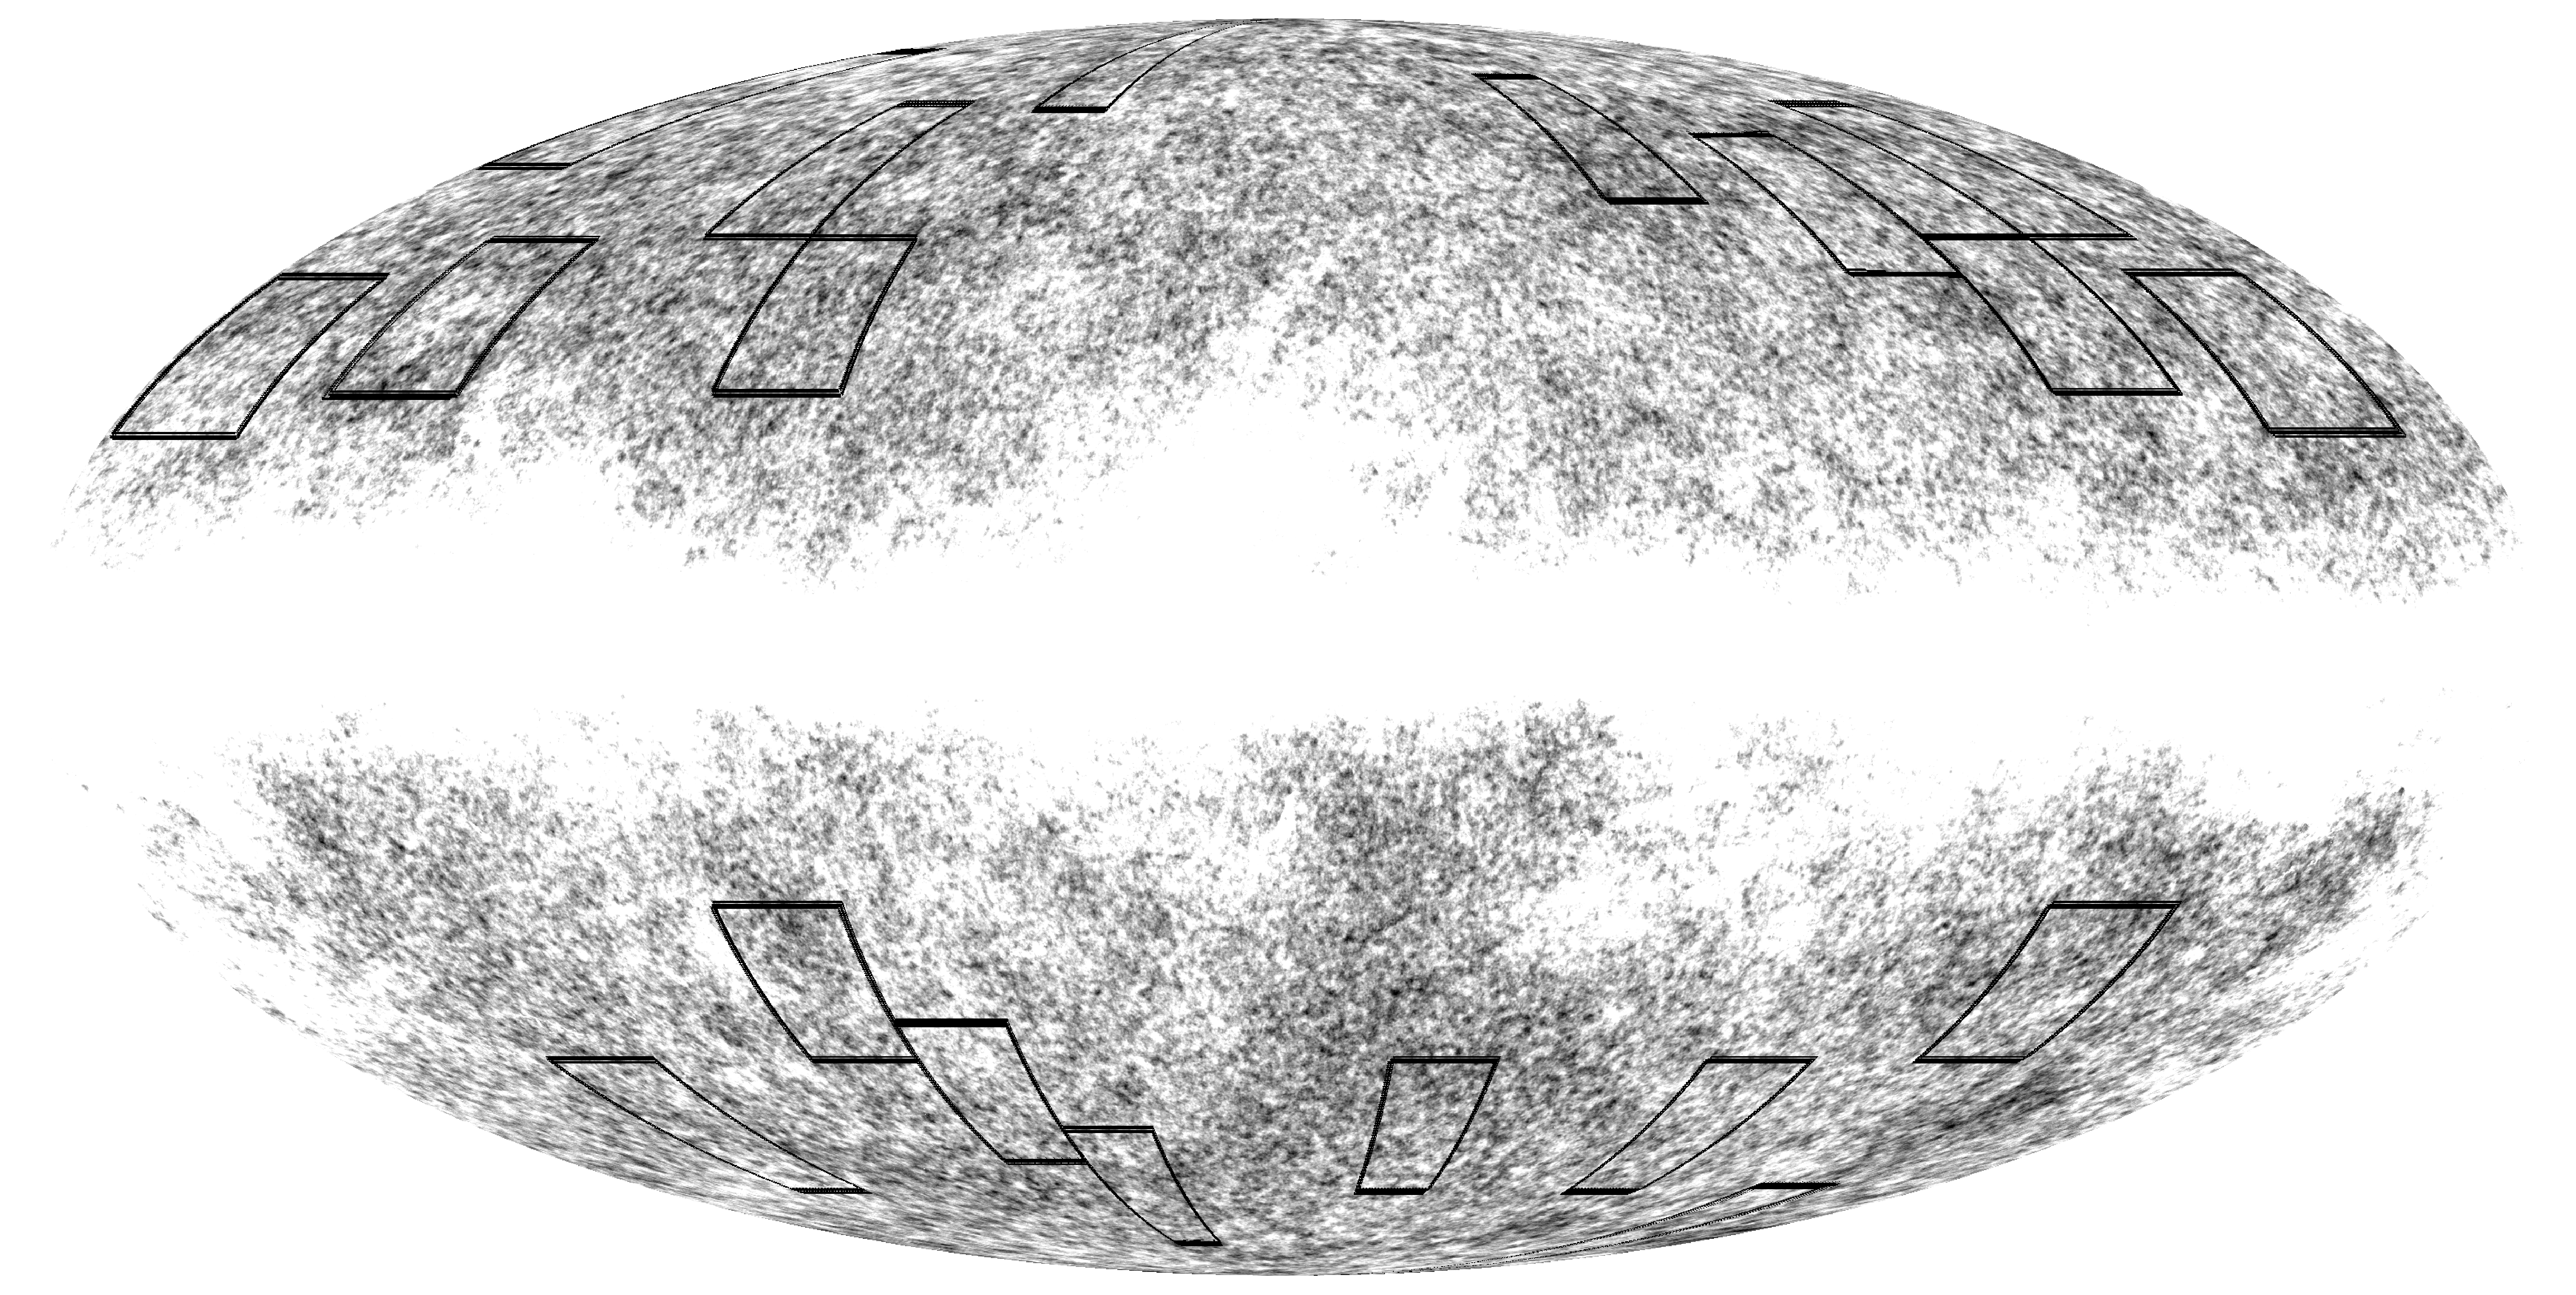
\includegraphics[width=0.9\textwidth]{areas_217_wb}} 
		\end{tabular}
		\caption{Расположение областей размером $20\degree \times 20\degree$ на картах частотами 30 MHz и 217 MHz}
		\label{areas}
		\end{center}
	\end{figure}

\newpage
\section{Калибровка}
	\begin{figure}[h!]
		\begin{tabular}{ccc}
			\subfloat[30 MHz $a=3.30$]{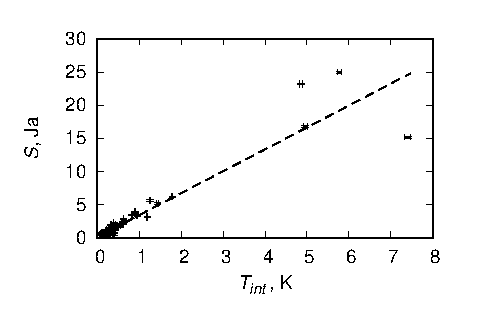
\includegraphics[width=0.33\textwidth]{030_0_wb}} &
			\subfloat[44 MHz $a=4.72$]{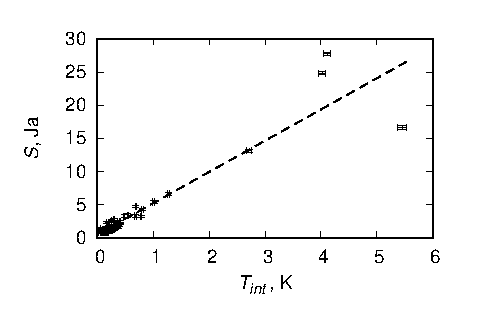
\includegraphics[width=0.33\textwidth]{044_0_wb}} &
			\subfloat[70 MHz $a=12.4$]{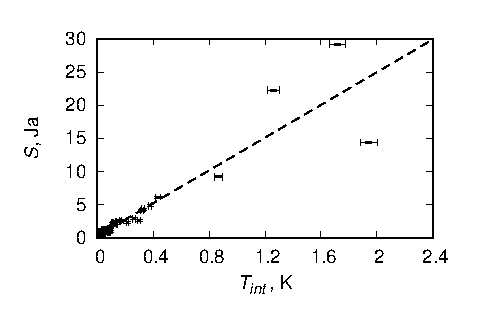
\includegraphics[width=0.33\textwidth]{070_0_wb}} \\
			\subfloat[100 MHz $a=20.6$]{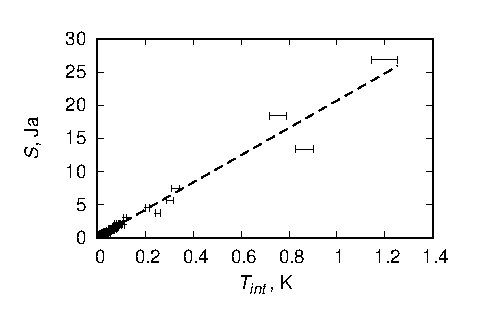
\includegraphics[width=0.33\textwidth]{100_0_wb}} &
			\subfloat[143 MHz $a=30.6$]{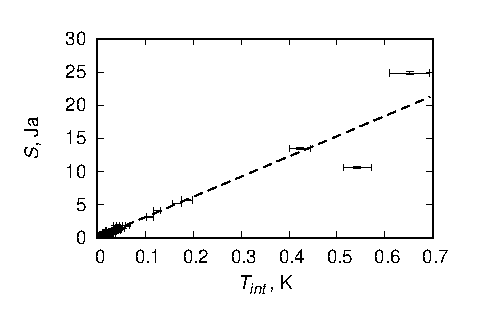
\includegraphics[width=0.33\textwidth]{143_0_wb}} &
			\subfloat[217 MHz $a=35.7$]{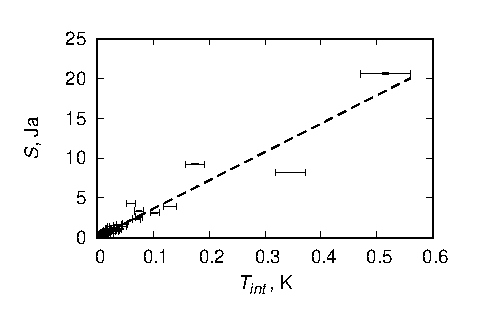
\includegraphics[width=0.33\textwidth]{217_0_wb}} 
		\end{tabular}
		\caption{Зависимости плотности потока для источников из каталога Planck от интегральной интенсивности, измеренной по картам микроволнового излучения миссии Planck изофото-скорректированным методом, реализованным программой \texttt{SExtractor}, и калибровочные прямые; $a$ --- угловой коэффициент калибровочной прямой. Использована выборка порядка 100 источников}
		\label{calib_0}
	\end{figure}

	\begin{figure}
		\begin{tabular}{ccc}
			\subfloat[30 MHz]{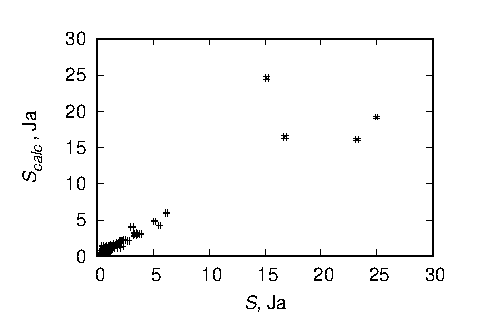
\includegraphics[width=0.33\textwidth]{corr_030_0_wb}} &
			\subfloat[44 MHz]{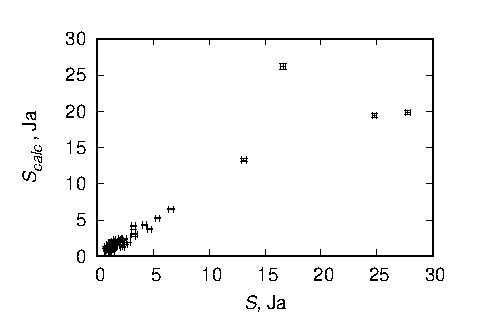
\includegraphics[width=0.33\textwidth]{corr_044_0_wb}} &
			\subfloat[70 MHz]{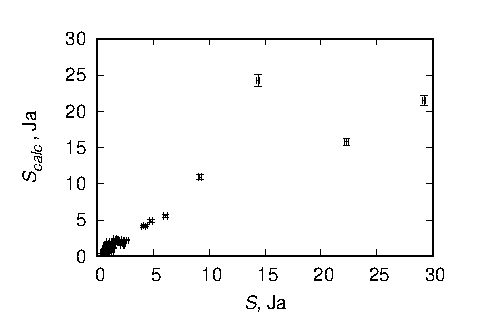
\includegraphics[width=0.33\textwidth]{corr_070_0_wb}} \\
			\subfloat[100 MHz]{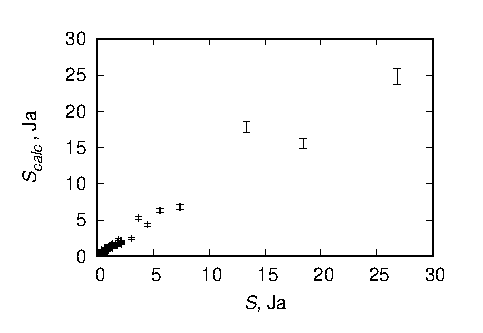
\includegraphics[width=0.33\textwidth]{corr_100_0_wb}} &
			\subfloat[143 MHz]{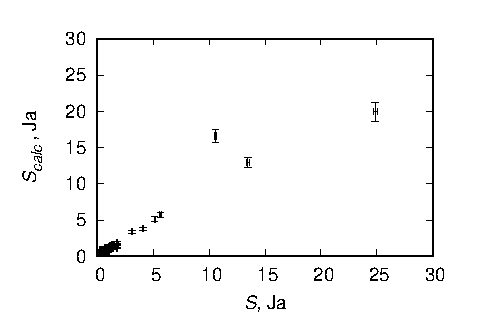
\includegraphics[width=0.33\textwidth]{corr_143_0_wb}} &
			\subfloat[217 MHz]{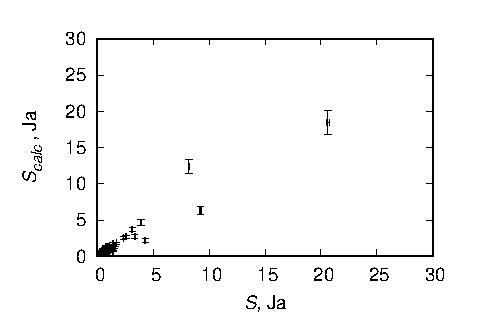
\includegraphics[width=0.33\textwidth]{corr_217_0_wb}} 
		\end{tabular}
		\caption{Зависимости плотности потока для источников из каталога Planck от плотности потока, рассчитанной из интегральной интенсивности, измеренной по картам микроволнового излучения}
		\label{corr_0}
	\end{figure}

	\begin{figure}
		\begin{tabular}{ccc}
			\subfloat[30 MHz --- 5 arcmin \newline $a=3.21$]{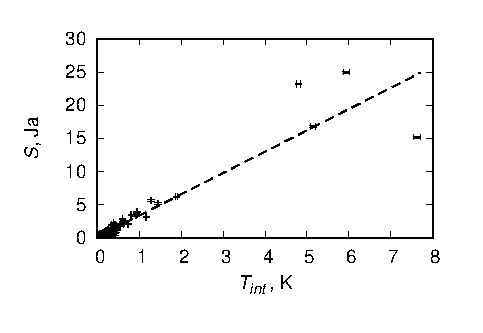
\includegraphics[width=0.33\textwidth]{030_5_wb}} &
			\subfloat[30 MHz --- 35 arcmin \newline $a=190$]{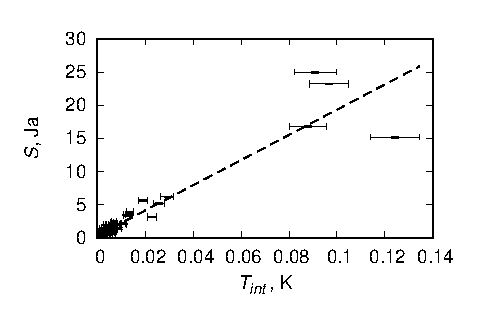
\includegraphics[width=0.33\textwidth]{030_35_wb}} &
			\subfloat[30 MHz --- 60 arcmin \newline $a=323$]{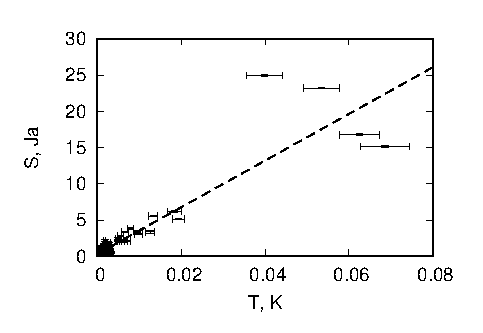
\includegraphics[width=0.33\textwidth]{030_60_wb}} \\
			\subfloat[30 MHz --- 5 arcmin]{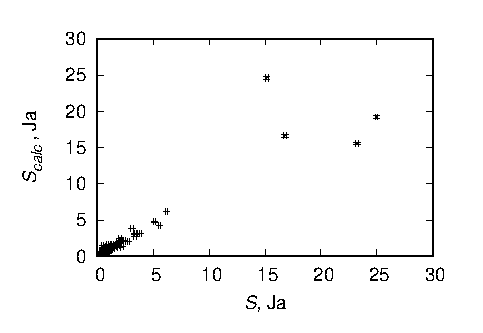
\includegraphics[width=0.33\textwidth]{corr_030_5_wb}} &
			\subfloat[30 MHz --- 35 arcmin]{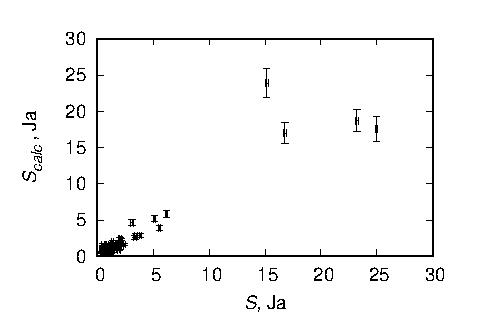
\includegraphics[width=0.33\textwidth]{corr_030_35_wb}} &
			\subfloat[30 MHz --- 60 arcmin]{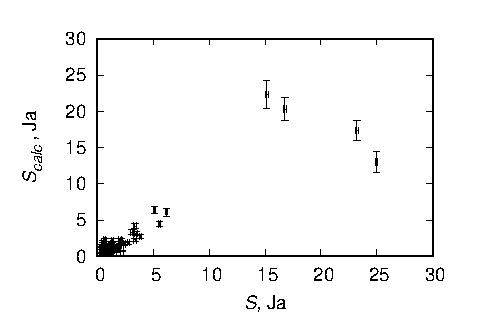
\includegraphics[width=0.33\textwidth]{corr_030_60_wb}} 
		\end{tabular}
		\caption{a, b, c: зависимости плотности потока на частоте $30$ MHz для источников из каталога Planck от интегральной интенсивности, измеренной по картам микроволнового излучения для различных угловых размеров сглаживания карты; $a$ --- угловой коэффициент калибровочной прямой\\ d, e, f: зависимости плотности потока для источников из каталога Planck от плотности потока, рассчитанной из интегральной интенсивности, измеренной по сглаженным картам микроволнового излучения}
		\label{calib_corr_030_conv}
	\end{figure}

	\begin{figure}
		\begin{tabular}{ccc}
			\subfloat[44 MHz --- 5 arcmin \newline $a=5.82$]{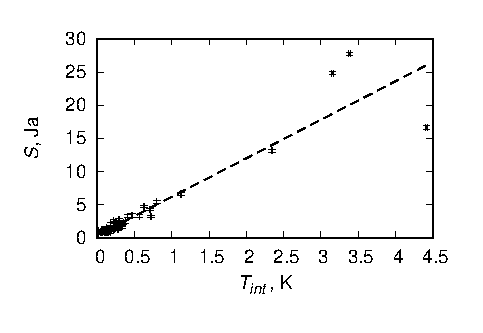
\includegraphics[width=0.33\textwidth]{044_5_wb}} &
			\subfloat[44 MHz --- 35 arcmin \newline $a=402$]{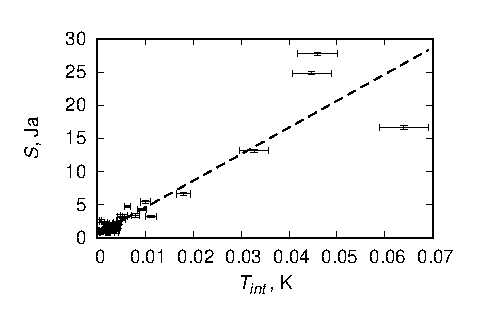
\includegraphics[width=0.33\textwidth]{044_35_wb}} &
			\subfloat[44 MHz --- 60 arcmin \newline $a=651$]{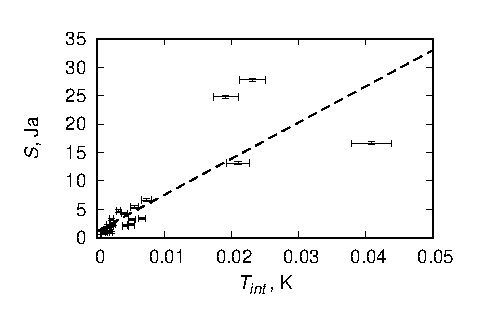
\includegraphics[width=0.33\textwidth]{044_60_wb}} \\
			\subfloat[44 MHz --- 5 arcmin]{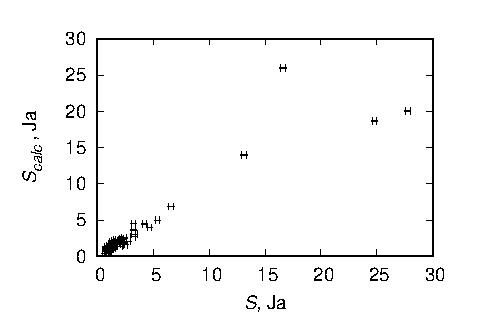
\includegraphics[width=0.33\textwidth]{corr_044_5_wb}} &
			\subfloat[44 MHz --- 35 arcmin]{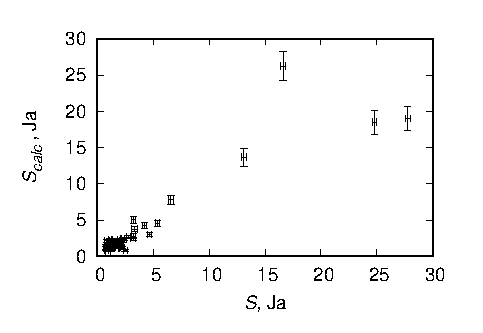
\includegraphics[width=0.33\textwidth]{corr_044_35_wb}} &
			\subfloat[44 MHz --- 60 arcmin]{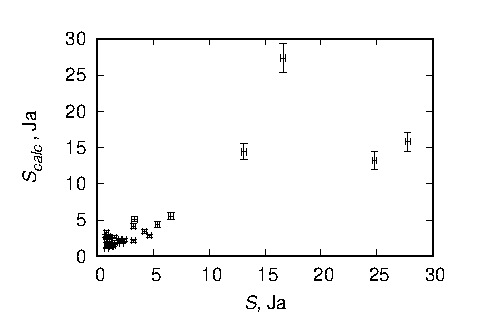
\includegraphics[width=0.33\textwidth]{corr_044_60_wb}} 
		\end{tabular}
		\caption{a, b, c: зависимости плотности потока на частоте $44$ MHz для источников из каталога Planck от интегральной интенсивности, измеренной по картам микроволнового излучения для различных угловых размеров сглаживания карты; $a$ --- угловой коэффициент калибровочной прямой\\ d, e, f: зависимости плотности потока для источников из каталога Planck от плотности потока, рассчитанной из интегральной интенсивности, измеренной по сглаженным картам микроволнового излучения}
		\label{calib_corr_044_conv}
	\end{figure}

	\begin{figure}
		\begin{tabular}{ccc}
			\subfloat[70 MHz --- 5 arcmin \newline $a=13.1$]{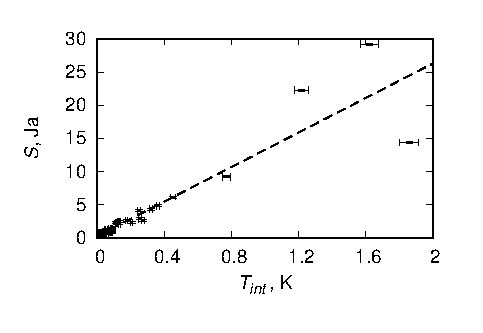
\includegraphics[width=0.33\textwidth]{070_5_wb}} &
			\subfloat[70 MHz --- 35 arcmin \newline $a=573$]{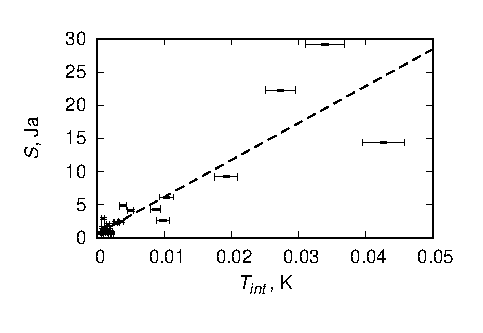
\includegraphics[width=0.33\textwidth]{070_35_wb}} &
			\subfloat[70 MHz --- 60 arcmin \newline $a=1510$]{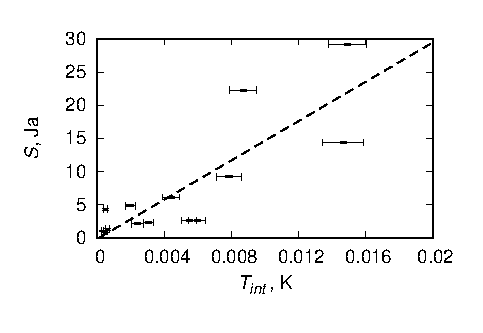
\includegraphics[width=0.33\textwidth]{070_60_wb}} \\
			\subfloat[70 MHz --- 5 arcmin]{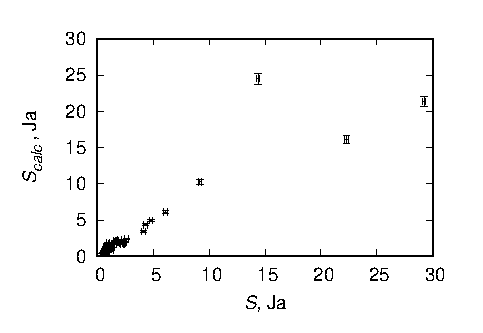
\includegraphics[width=0.33\textwidth]{corr_070_5_wb}} &
			\subfloat[70 MHz --- 35 arcmin]{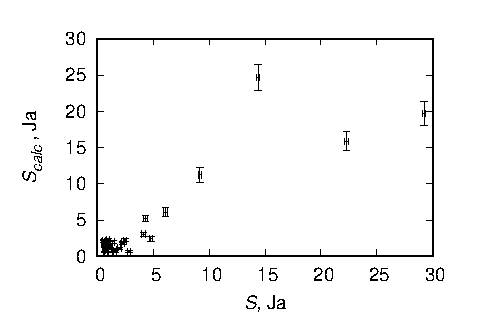
\includegraphics[width=0.33\textwidth]{corr_070_35_wb}} &
			\subfloat[70 MHz --- 60 arcmin]{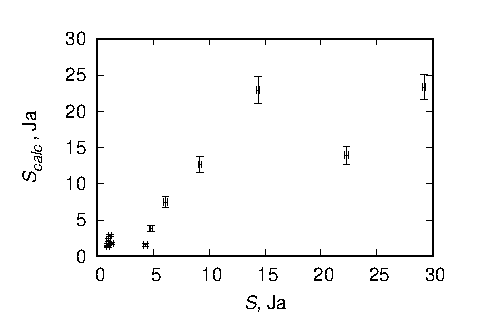
\includegraphics[width=0.33\textwidth]{corr_070_60_wb}} 
		\end{tabular}
		\caption{a, b, c: зависимости плотности потока на частоте $70$ MHz для источников из каталога Planck от интегральной интенсивности, измеренной по картам микроволнового излучения для различных угловых размеров сглаживания карты; $a$ --- угловой коэффициент калибровочной прямой\\ d, e, f: зависимости плотности потока для источников из каталога Planck от плотности потока, рассчитанной из интегральной интенсивности, измеренной по сглаженным картам микроволнового излучения}
		\label{calib_corr_070_conv}
	\end{figure}

	\begin{figure}
		\begin{tabular}{ccc}
			\subfloat[100 MHz --- 5 arcmin \newline $a=25.2$]{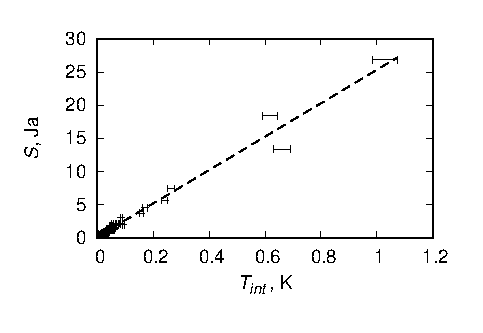
\includegraphics[width=0.33\textwidth]{100_5_wb}} &
			\subfloat[100 MHz --- 35 arcmin \newline $a=908$]{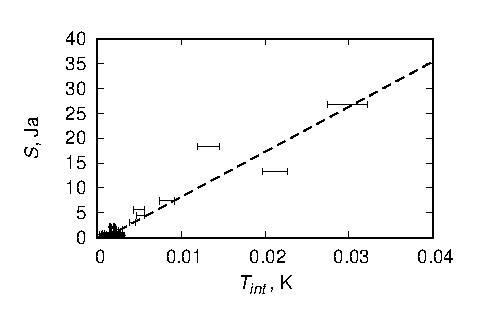
\includegraphics[width=0.33\textwidth]{100_35_wb}} &
			\subfloat[100 MHz --- 60 arcmin \newline $a=2740$]{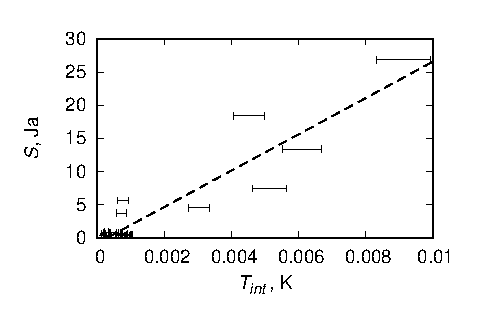
\includegraphics[width=0.33\textwidth]{100_60_wb}} \\
			\subfloat[100 MHz --- 5 arcmin]{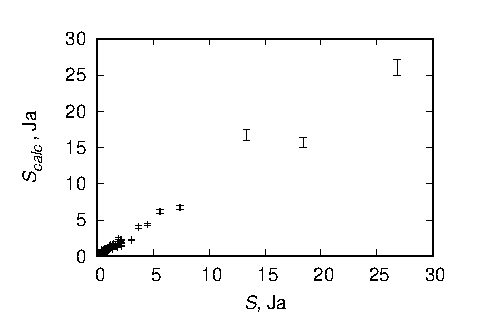
\includegraphics[width=0.33\textwidth]{corr_100_5_wb}} &
			\subfloat[100 MHz --- 35 arcmin]{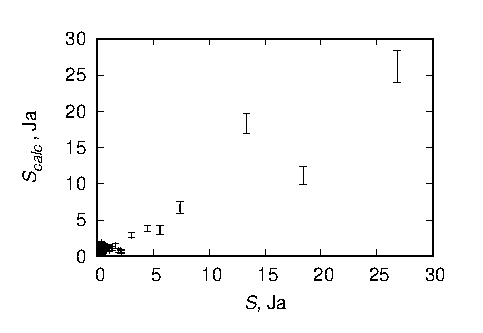
\includegraphics[width=0.33\textwidth]{corr_100_35_wb}} &
			\subfloat[100 MHz --- 60 arcmin]{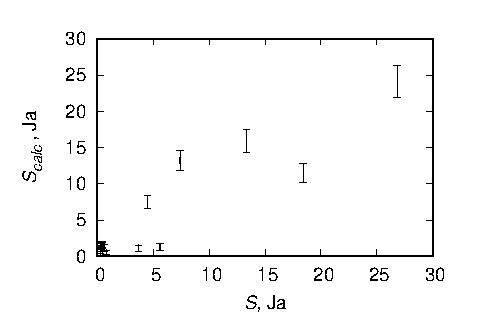
\includegraphics[width=0.33\textwidth]{corr_100_60_wb}} 
		\end{tabular}
		\caption{a, b, c: зависимости плотности потока на частоте $100$ MHz для источников из каталога Planck от интегральной интенсивности, измеренной по картам микроволнового излучения для различных угловых размеров сглаживания карты; $a$ --- угловой коэффициент калибровочной прямой\\ d, e, f: зависимости плотности потока для источников из каталога Planck от плотности потока, рассчитанной из интегральной интенсивности, измеренной по сглаженным картам микроволнового излучения}
		\label{calib_corr_100_conv}
	\end{figure}
	
	\begin{figure}
		\begin{tabular}{ccc}
			\subfloat[143 MHz --- 5 arcmin \newline $a=54.4$]{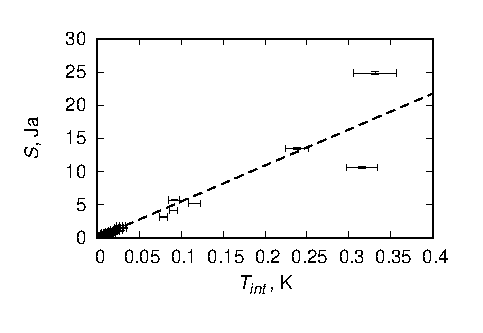
\includegraphics[width=0.33\textwidth]{143_5_wb}} &
			\subfloat[143 MHz --- 35 arcmin \newline $a=1220$]{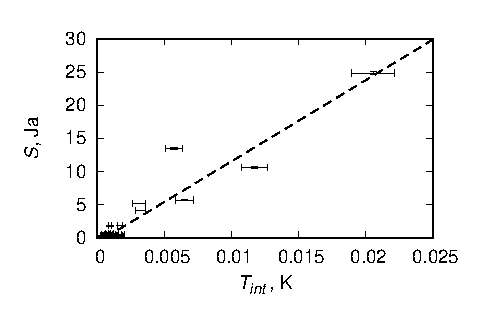
\includegraphics[width=0.33\textwidth]{143_35_wb}} &
			\subfloat[143 MHz --- 60 arcmin \newline $a=2910$]{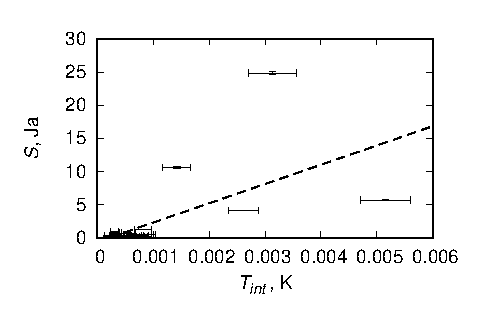
\includegraphics[width=0.33\textwidth]{143_60_wb}} \\
			\subfloat[143 MHz --- 5 arcmin]{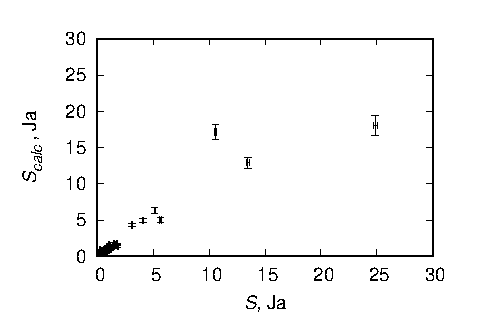
\includegraphics[width=0.33\textwidth]{corr_143_5_wb}} &
			\subfloat[143 MHz --- 35 arcmin]{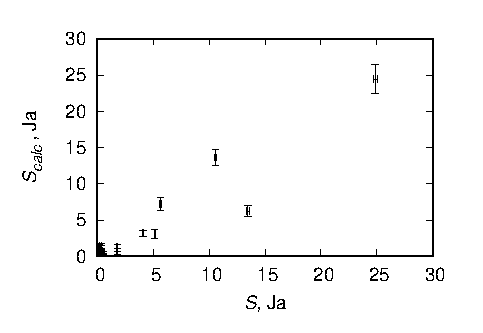
\includegraphics[width=0.33\textwidth]{corr_143_35_wb}} &
			\subfloat[143 MHz --- 60 arcmin]{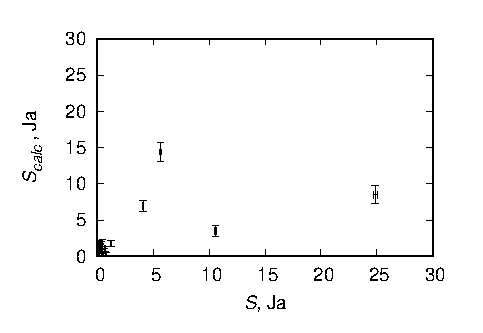
\includegraphics[width=0.33\textwidth]{corr_143_60_wb}} 
		\end{tabular}
		\caption{a, b, c: зависимости плотности потока на частоте $143$ MHz для источников из каталога Planck от интегральной интенсивности, измеренной по картам микроволнового излучения для различных угловых размеров сглаживания карты; $a$ --- угловой коэффициент калибровочной прямой\\ d, e, f: зависимости плотности потока для источников из каталога Planck от плотности потока, рассчитанной из интегральной интенсивности, измеренной по сглаженным картам микроволнового излучения}
		\label{calib_corr_143_conv}
	\end{figure}
	
	\begin{figure}
		\begin{tabular}{ccc}
			\subfloat[217 MHz --- 5 arcmin \newline $a=114$]{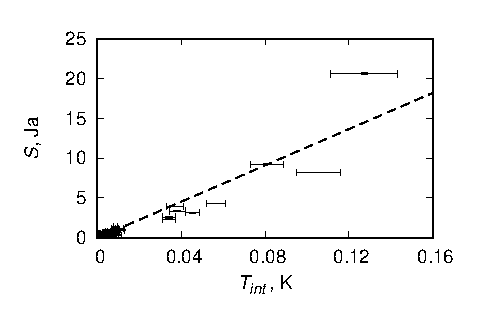
\includegraphics[width=0.33\textwidth]{217_5_wb}} &
			\subfloat[217 MHz --- 35 arcmin \newline $a=1480$]{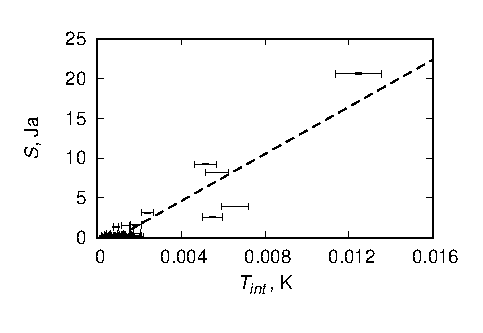
\includegraphics[width=0.33\textwidth]{217_35_wb}} &
			\subfloat[217 MHz --- 60 arcmin \newline ???$a=1300$]{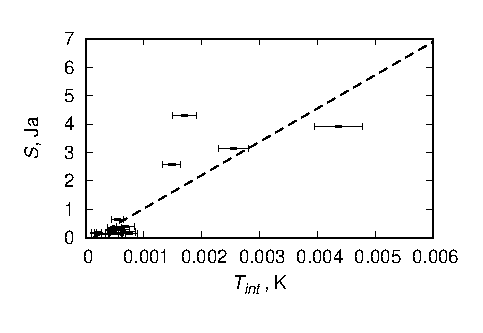
\includegraphics[width=0.33\textwidth]{217_60_wb}} \\
			\subfloat[217 MHz --- 5 arcmin]{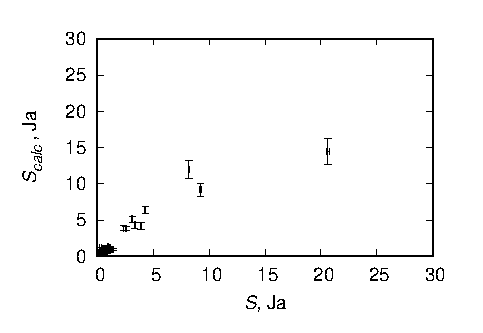
\includegraphics[width=0.33\textwidth]{corr_217_5_wb}} &
			\subfloat[217 MHz --- 35 arcmin]{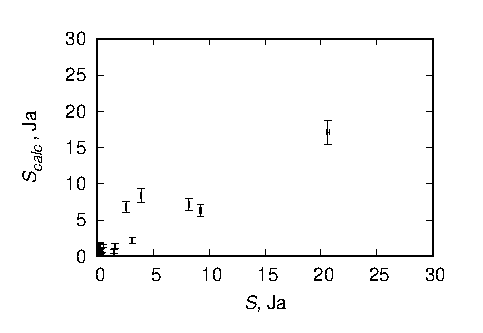
\includegraphics[width=0.33\textwidth]{corr_217_35_wb}} &
			\subfloat[217 MHz --- 60 arcmin]{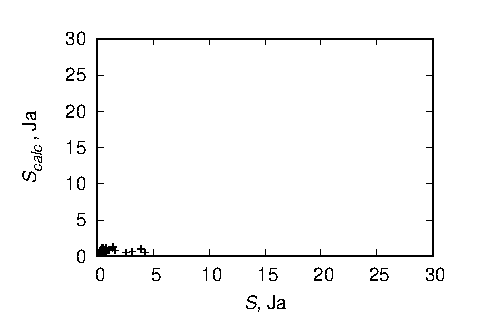
\includegraphics[width=0.33\textwidth]{corr_217_60_wb}} 
		\end{tabular}
		\caption{a, b, c: зависимости плотности потока на частоте $217$ MHz для источников из каталога Planck от интегральной интенсивности, измеренной по картам микроволнового излучения для различных угловых размеров сглаживания карты; $a$ --- угловой коэффициент калибровочной прямой\\ d, e, f: зависимости плотности потока для источников из каталога Planck от плотности потока, рассчитанной из интегральной интенсивности, измеренной по сглаженным картам микроволнового излучения}
		\label{calib_corr_217_conv}
	\end{figure}

\begin{table}[h!]
	\setcaptionmargin{0mm}
	\caption{Параметры калибровочных кривых. Здесь $cr$ --- угловой размер сглаживания, $\sigma_a$ --- относительная ошибка определения углового коэффициента прямой, $N_s$ --- размер выборки источников из каталога}
	\label{tab:calib}
	\medskip
	\begin{tabular}{c|c|c|c|c}
		$f$, MHz & $cr$, arcmin & $S$, Jy & $\sigma_a$ & $N_s$\\[3 pt] \hline
		30 & 0 & $3.3093T+0.0897$ & 3\% & 200\\[3 pt]
		30 & 5 & $3.2165T+0.1090$ & 3\% & 200\\[3 pt]
		30 & 35 & $190.2627T+0.2905$ & 3\% & 100\\[3 pt]
		30 & 60 & $323.4203T+0.1216$ & 5\% & 100\\[3 pt]
		44 & 0 & $4.7156T+0.4843$ & 4\% & 100\\[3 pt]
		44 & 5 & $5.8174T+0.3454$ & 4\% & 100\\[3 pt]
		44 & 35 & $402.4858T+0.5232$ & 6\% & 50\\[3 pt]
		44 & 60 & $650.6276T+0.7825$ & 13\% & 30\\[3 pt]
		70 & 0 & $12.4071T+0.1766$ & 4\% & 100\\[3 pt]
		70 & 5 & $13.0744T+0.1893$ & 4\% & 100\\[3 pt]
		70 & 35 & $573.8741T+0.1928$& 9\% & 35\\[3 pt]
		70 & 60 & $1507.0105T+0.8544$ & 16\% & 12\\[3 pt]
		100 & 0 & $20.5963T+0.0809$ & 1\% & 250\\[3 pt]
		100 & 5 & $25.2404T+0.1008$ & 1\% & 200\\[3 pt]
		100 & 35 & $907.5971T-0.8944$ & 4\% & 50\\[3 pt]
		100 & 60 & $2738.5083T-0.8365$ & 8\% & 25\\[3 pt]
		143 & 0 & $30.5618T+0.0293$ & 1.5\% & 250\\[3 pt]
		143 & 5 & $54.3722T+0.0085$ & 3\% & 200\\[3 pt]
		143 & 35 & $1224.9972T-0.7364$ & 6\% & 34\\[3 pt]
		143 & 60 & $2910.8894T-0.6412$ & 30\% & 22\\[3 pt]
		217 & 0 & $35.7290T+0.0489$ & 1.5\% & 350\\[3 pt]
		217 & 5 & $114.1688T-0.0503$ & 2\% & 250\\[3 pt]
		217 & 35 & $1482.8214T-1.3392$ & 6\% & 48\\[3 pt]
		217 & 60 & $1174.8671T-0.1534$ & 15\% & 19\\[3 pt]
	\end{tabular}
\end{table}

\newpage
\section{Спектры пятен}

\begin{table}[h!]
	\setcaptionmargin{0mm}
	\caption{Размеры выборок пятен микроволнового фона, использованных для построения спектров}
	\label{tab:nums_spectr}
	\medskip
	\begin{tabular}{c|c|c}
		$cr$, arcmin & тип спектра: с амплитудами & тип спектра: с плотностями потока \\[3 pt] \hline
		0 & 12000 & 19400 \\[3 pt]
		5 & 5100 & 8850 \\[3 pt]
		35 & 480 & 680 \\[3 pt]
		60 & 315 & 360 \\[3 pt]
	\end{tabular}
\end{table}

	\begin{figure}[h!]
		\begin{tabular}{cc}
			\subfloat[0 arcmin]{\includegraphics[width=0.5\textwidth]{a_0_wb}} &
			\subfloat[5 arcmin]{\includegraphics[width=0.5\textwidth]{a_5_wb}} \\
			\subfloat[35 arcmin]{\includegraphics[width=0.5\textwidth]{a_35_wb}} &
			\subfloat[60 arcmin]{\includegraphics[width=0.5\textwidth]{a_60_wb}} 
		\end{tabular}
		\caption{Усредненный спектр пятен из карты SMICA, построенный по картам различного углового размера сглаживания; по вертикальной оси отложены амплитуды}
		\label{spectrum_amplitude}
	\end{figure}

	\begin{figure}
		\begin{tabular}{cc}
			\subfloat[0 arcmin]{\includegraphics[width=0.5\textwidth]{0_wb}} &
			\subfloat[5 arcmin]{\includegraphics[width=0.5\textwidth]{5_wb}} \\
			\subfloat[35 arcmin]{\includegraphics[width=0.5\textwidth]{35_wb}} &
			\subfloat[60 arcmin]{\includegraphics[width=0.5\textwidth]{60_wb}} 
		\end{tabular}
		\caption{Откалиброванный усредненный спектр пятен из карты SMICA, построенный по картам различного углового размера сглаживания; по вертикальной оси отложены плотности потока}
		\label{spectrum_calibrated}
	\end{figure}

\newpage
\section{Список использованных для построения калибровочных прямых источников из каталога Planck}

$f = 30$ MHz, $cr = 0$ arcmin 
\begin{multicols}{\numofcol}
\raggedright
\footnotesize
G113.07-56.57, G116.49-52.02, G115.13-64.85, G122.71-69.70, G126.62-64.33, G127.42-68.55, G126.71-62.69, G170.90-85.80, G215.80-86.67, G131.84-60.98, G276.21-80.11, G133.99-59.93, G136.32-63.73, G136.08-59.16, G172.99-81.67, G213.88-83.53, G134.59-50.34, G137.29-57.65, G141.23-61.79, G261.69-77.07, G201.31-79.27, G218.13-78.08, G240.49-75.52, G280.69-63.24, G272.80-66.99, G276.08-61.76, G261.89-60.13, G258.59-61.02, G272.49-54.60, G241.27-48.92, G231.26-48.49, G221.00-47.02, G237.75-48.48, G241.26-47.90, G233.41-47.49, G216.87-43.12, G240.49-44.67, G240.72-43.60, G229.02-37.01, G234.41-34.18, G223.56-30.78, G164.21+30.56, G170.52+30.20, G197.91+26.40, G174.74+31.71, G179.64+31.45, G169.19+32.67, G171.12+33.19, G202.29+27.71, G178.26+33.40, G201.33+29.67, G200.04+31.88, G162.17+36.53, G158.53+36.55, G207.31+32.56, G206.82+35.81, G205.66+36.68, G173.04+41.54, G197.08+40.61, G228.96+30.94, G228.30+32.85, G134.21+33.73, G152.23+41.00, G198.82+44.43, G232.50+33.70, G228.58+42.27, G236.58+38.74, G141.43+40.58, G194.29+52.32, G145.78+43.13, G199.60+52.63, G242.77+40.82, G243.50+41.61, G207.64+54.60, G210.65+54.43, G227.06+50.86, G149.01+47.28, G228.33+53.16, G248.12+44.44, G241.66+51.57, G252.07+46.08, G241.05+52.67, G211.56+60.99, G224.55+59.47, G252.81+50.69, G222.56+63.12, G251.50+52.76, G189.91+66.97, G260.95+52.10, G242.27+63.94, G256.05+60.92, G174.43+69.81, G268.88+52.56, G270.36+53.46, G165.00+71.46, G272.58+58.80, G160.72+72.03, G280.98+55.34, G280.77+59.81, G285.40+61.19, G281.81+67.38, G287.98+59.23, G284.71+66.05, G278.39+74.46, G289.94+64.37, G283.76+74.50, G293.12+60.05, G293.95+70.14, G305.12+57.06, G101.33+80.63, G085.75+83.29, G102.62+78.03, G086.99+80.83, G359.46+81.68, G067.31+81.12, G003.38+80.50, G107.77+65.96, G064.56+80.32, G022.29+80.95, G056.54+80.65, G036.94+80.75, G112.31+57.54, G100.54+69.49, G109.32+60.85, G104.86+61.40, G021.68+76.29, G054.74+76.05, G080.22+70.76, G109.56+53.07, G097.51+60.77, G086.68+64.59, G098.27+58.31, G092.98+60.55, G088.02+59.21, G090.54+57.52, G076.28+44.53, G087.58+42.07, G076.51+42.81, G073.40+41.88, G086.64+40.35, G089.62+37.46, G085.80+37.85, G073.79+38.44, G075.68-29.64, G064.60-38.61, G044.88-50.29, G078.32-30.04, G077.06-33.55, G059.00-46.65, G083.17-30.08, G058.96-48.85, G055.24-51.70, G077.44-38.58, G078.15-41.45, G053.88-57.06, G013.97-62.95, G023.65-63.31, G086.10-38.18, G084.42-40.27, G041.56-62.86, G080.45-45.42, G075.78-49.57, G024.42-64.92, G088.37-38.30, G071.82-53.49, G045.77-63.73, G085.35-45.30, G014.91-68.53, G334.67-60.50, G085.46-50.91, G077.75-58.20, G080.57-57.70, G061.19-67.07, G332.01-62.31, G335.67-64.07, G059.83-68.41, G039.62-72.17, G326.70-60.82, G065.60-70.91, G065.56-71.93, G326.99-64.37, G320.15-62.09, G314.06-55.08, G008.02-77.87
\end{multicols}

$f = 44$ MHz, $cr = 0$ arcmin
\begin{multicols}{\numofcol}
\raggedright
\footnotesize 
G112.98-56.55, G115.09-64.80, G122.51-69.69, G126.47-64.40, G170.50-85.85, G131.84-60.97, G134.60-50.37, G141.22-61.83, G201.27-79.28, G215.76-78.78, G218.25-78.05, G207.72-72.73, G276.05-61.78, G272.46-54.61, G237.73-48.49, G241.26-47.92, G240.65-44.47, G240.73-43.59, G229.03-37.02, G223.65-34.92, G234.46-34.17, G170.60+30.20, G179.64+31.46, G178.23+33.37, G200.04+31.89, G206.81+35.81, G228.98+30.90, G152.29+40.96, G198.83+44.43, G232.47+33.66, G141.48+40.58, G145.79+43.06, G241.63+51.51, G241.17+52.68, G239.85+53.39, G252.74+50.88, G251.53+52.78, G203.88+66.64, G174.48+69.81, G182.64+71.64, G164.85+71.47, G280.92+59.88, G281.77+67.38, G288.15+59.24, G284.83+66.05, G289.93+64.35, G283.79+74.50, G293.08+60.17, G305.11+57.06, G101.33+80.63, G085.47+83.31, G003.24+80.46, G056.47+80.67, G047.20+71.09, G098.32+58.30, G090.48+57.52, G073.39+41.93, G086.67+40.34, G067.66+37.71, G075.65-29.60, G059.04-46.61, G083.16-30.09, G058.98-48.84, G055.22-51.71, G077.44-38.59, G053.85-57.03, G023.96-63.23, G086.12-38.19, G084.38-40.27, G024.40-64.91, G071.81-53.41, G334.48-60.50, G085.59-50.82, G077.83-58.30, G332.04-62.32, G335.52-64.09, G039.56-72.20, G065.65-71.93, G320.17-62.04, G314.09-55.08
\end{multicols}

$f = 70$ MHz, $cr = 0$ arcmin
\begin{multicols}{\numofcol}
\raggedright
\footnotesize 
G115.22-64.81, G118.22-55.14, G122.76-69.72, G170.74-85.78, G216.04-86.68, G131.79-60.99, G173.22-81.73, G134.65-50.34, G137.36-57.66, G139.36-51.15, G201.31-79.28, G217.99-78.15, G276.08-61.76, G262.73-64.09, G258.65-61.06, G261.81-60.12, G272.46-54.60, G231.24-48.46, G237.73-48.46, G241.31-47.87, G240.68-44.39, G240.69-43.61, G228.25-40.31, G239.47-39.86, G229.03-36.99, G234.35-34.15, G170.63+30.16, G178.24+33.37, G200.03+31.87, G206.80+35.82, G173.02+41.59, G228.93+30.92, G196.23+42.07, G228.32+32.79, G152.19+41.02, G198.90+44.41, G141.40+40.54, G145.75+43.13, G228.35+53.21, G248.07+44.53, G241.65+51.54, G241.05+52.62, G211.66+60.99, G251.49+52.78, G196.97+65.53, G240.56+60.58, G186.99+67.54, G157.53+64.25, G197.56+72.05, G174.54+69.82, G268.89+52.53, G266.46+55.91, G164.90+71.45, G281.77+67.40, G284.76+66.05, G289.90+64.36, G283.67+74.50, G305.12+57.07, G108.29+84.51, G101.04+80.64, G085.70+83.35, G358.46+81.74, G003.28+80.50, G022.13+80.98, G056.70+80.65, G054.31+76.10, G109.54+53.20, G098.30+58.32, G088.08+59.19, G090.49+57.54, G090.73+40.16, G073.44+41.90, G086.65+40.34, G075.67-29.65, G068.51-38.82, G059.04-46.63, G083.20-30.09, G058.96-48.85, G047.84-56.20, G078.11-41.45, G053.87-57.06, G013.71-62.88, G086.41-37.50, G086.09-38.18, G084.41-40.27, G071.89-53.50, G014.96-68.52, G085.46-50.93, G077.70-58.23, G335.71-64.04, G331.95-62.30, G039.62-72.18, G065.89-70.98, G065.54-71.90, G328.86-68.43, G320.14-62.10, G314.10-55.08
\end{multicols}

$f = 100$ MHz, $cr = 0$ arcmin
\begin{multicols}{\numofcol}
\raggedright
\footnotesize 
G112.71-53.14, G114.77-63.79, G115.22-64.77, G116.74-64.50, G122.72-69.71, G170.40-85.80, G216.64-86.66, G131.78-60.98, G204.05-85.52, G276.11-80.08, G134.13-60.01, G169.64-81.52, G173.38-81.69, G213.52-83.52, G228.61-83.17, G134.59-50.36, G137.28-57.65, G141.08-61.74, G174.67-76.26, G201.40-79.27, G239.43-77.77, G218.08-78.08, G246.88-75.16, G221.01-76.35, G241.03-75.37, G240.99-73.15, G276.06-61.77, G235.29-70.70, G201.49-68.79, G265.96-62.96, G262.80-64.00, G266.29-61.64, G258.54-61.04, G261.83-60.10, G257.57-60.99, G272.51-54.59, G231.22-48.51, G220.99-46.97, G237.73-48.49, G241.28-47.87, G236.44-44.70, G240.67-44.39, G240.71-43.62, G234.10-39.51, G224.22-36.35, G229.01-37.00, G233.50-37.07, G223.70-34.90, G234.40-34.16, G227.64-32.52, G178.46+28.35, G164.22+30.51, G170.52+30.14, G169.16+32.56, G179.65+31.45, G178.90+31.94, G178.23+33.40, G189.82+31.64, G178.34+33.74, G180.35+34.03, G201.35+29.66, G161.99+35.12, G191.99+32.93, G200.02+31.89, G170.12+36.38, G178.60+36.27, G158.67+36.60, G170.46+39.26, G167.58+39.13, G206.80+35.82, G190.70+40.38, G173.05+41.58, G226.85+30.78, G228.95+30.93, G228.37+32.83, G218.73+38.50, G152.20+40.96, G198.87+44.41, G217.85+41.73, G146.70+40.62, G221.42+45.06, G141.42+40.55, G145.73+43.13, G199.50+52.61, G234.64+44.77, G231.59+46.20, G243.42+40.37, G233.49+46.01, G217.83+52.00, G210.10+53.92, G210.67+54.45, G227.02+50.74, G250.52+41.68, G228.33+53.14, G248.05+44.52, G241.72+51.55, G241.09+52.64, G211.57+60.98, G234.07+56.42, G224.39+59.39, G245.47+53.35, G251.49+52.77, G198.99+66.12, G179.85+65.01, G253.14+54.36, G204.08+66.66, G186.92+67.56, G263.70+51.41, G242.20+63.93, G266.22+50.45, G174.50+69.79, G268.95+52.51, G270.08+53.52, G262.91+64.18, G164.91+71.45, G160.55+72.02, G162.01+73.49, G268.59+66.81, G280.54+54.99, G281.16+55.30, G143.84+67.07, G266.09+71.81, G280.70+59.86, G281.75+67.37, G285.00+63.85, G284.81+66.04, G289.92+64.36, G290.68+63.84, G283.76+74.49, G286.79+71.66, G293.16+60.10, G294.08+70.14, G295.20+67.38, G301.58+56.34, G305.81+74.54, G305.09+57.07, G305.93+65.69, G108.39+84.46, G114.48+78.36, G101.23+80.62, G085.74+83.35, G086.04+83.08, G097.56+79.06, G086.89+80.78, G358.81+81.71, G003.36+80.51, G064.86+80.37, G056.57+80.66, G103.84+68.19, G037.02+80.71, G036.06+78.71, G105.79+61.75, G098.57+66.94, G104.90+61.37, G063.50+75.80, G051.38+76.54, G104.13+61.42, G054.64+76.09, G060.35+73.75, G047.37+73.42, G086.87+64.57, G082.32+66.09, G098.29+58.30, G092.95+60.53, G088.04+59.19, G090.51+57.49, G073.44+41.86, G086.61+40.34, G076.63+40.06, G089.60+37.43, G074.34+38.47, G073.71+38.44, G068.39+36.22, G075.47+34.95, G071.49+33.93, G075.65-29.63, G075.02-30.63, G076.10-30.75, G079.31-28.72, G044.86-50.28, G078.36-30.04, G069.76-37.61, G068.51-38.80, G052.80-48.92, G059.03-46.63, G044.84-53.31, G075.58-36.70, G083.16-30.08, G058.97-48.83, G055.20-51.70, G076.65-38.43, G077.44-38.59, G047.84-56.21, G078.15-39.76, G078.16-41.44, G048.19-58.49, G053.86-57.06, G331.94-53.37, G070.17-49.71, G013.78-62.91, G329.10-52.55, G086.11-38.17, G084.43-40.26, G041.54-62.88, G080.43-45.54, G334.30-56.66, G088.37-38.37, G071.86-53.50, G089.97-37.92, G089.17-40.93, G091.46-38.33, G065.67-60.20, G014.90-68.51, G334.68-60.50, G085.41-50.92, G333.90-61.29, G071.83-61.36, G077.75-58.20, G331.98-62.30, G335.72-64.07, G019.13-71.96, G060.01-68.38, G039.67-72.18, G338.27-66.60, G326.68-60.92, G065.69-70.96, G327.03-64.24, G065.48-71.89, G326.85-64.62, G330.98-68.23, G014.05-76.89, G316.36-57.50, G320.17-62.10, G328.76-68.44, G316.85-59.01
\end{multicols}

$f = 143$ MHz, $cr = 0$ arcmin
\begin{multicols}{\numofcol}
\raggedright
\footnotesize 
G114.75-63.78, G115.21-64.81, G117.03-61.30, G116.81-64.53, G120.19-59.94, G122.05-60.22, G122.72-69.71, G209.86-87.79, G170.79-85.82, G217.24-86.66, G133.37-65.88, G276.15-80.10, G134.12-60.01, G133.56-54.12, G169.70-81.53, G173.42-81.72, G213.64-83.54, G134.58-50.35, G137.27-57.64, G183.76-80.81, G141.34-58.57, G139.06-52.93, G201.41-79.28, G239.47-77.76, G218.11-78.09, G241.07-75.36, G276.06-61.77, G238.54-70.51, G216.27-70.93, G262.75-64.04, G266.28-61.64, G258.57-61.03, G261.82-60.08, G272.47-54.61, G231.22-48.51, G220.98-46.96, G237.73-48.48, G241.28-47.89, G216.91-43.18, G240.65-44.39, G240.69-43.62, G229.01-37.00, G223.69-34.87, G242.94-37.70, G234.42-34.17, G226.01-32.17, G170.60+29.41, G178.49+28.34, G170.54+30.13, G174.69+31.68, G169.16+32.57, G179.64+31.43, G204.24+25.55, G178.93+31.92, G160.34+33.17, G178.22+33.39, G189.81+31.65, G195.10+30.47, G165.40+34.75, G180.38+34.04, G201.35+29.68, G198.99+30.65, G161.93+35.13, G166.32+35.66, G200.02+31.87, G170.14+36.38, G178.58+36.25, G178.62+37.42, G170.49+39.24, G167.60+39.13, G206.82+35.83, G205.72+36.64, G173.03+41.55, G228.95+30.91, G191.93+42.09, G225.19+33.94, G228.33+32.81, G152.19+41.00, G198.85+44.39, G218.34+42.51, G221.42+45.06, G141.42+40.55, G194.18+52.32, G145.73+43.12, G199.48+52.62, G233.93+45.07, G233.50+46.00, G230.93+47.26, G243.40+41.61, G210.14+53.91, G210.68+54.42, G137.26+39.98, G227.04+50.75, G236.51+47.04, G235.12+48.19, G200.91+57.43, G210.83+56.81, G228.34+53.16, G248.07+44.51, G233.72+52.22, G134.20+39.19, G250.66+43.86, G237.90+51.71, G191.06+60.01, G214.84+58.99, G241.71+51.57, G241.10+52.66, G211.56+60.99, G245.49+53.34, G202.66+64.85, G251.48+52.77, G220.44+63.81, G179.85+65.02, G231.76+62.87, G253.15+54.34, G204.13+66.70, G240.18+62.32, G186.89+67.53, G248.08+60.76, G263.67+51.41, G242.28+63.91, G266.20+50.44, G168.63+67.13, G255.91+60.90, G268.47+52.12, G174.45+69.79, G268.93+52.52, G270.09+53.50, G262.47+61.14, G152.76+64.91, G272.56+53.52, G164.91+71.48, G268.96+64.58, G281.17+55.32, G143.76+67.08, G266.02+71.84, G280.67+59.88, G280.14+63.85, G141.48+69.08, G281.79+67.37, G284.77+66.05, G286.76+65.50, G278.25+74.48, G289.95+64.35, G283.75+74.49, G293.13+60.08, G294.91+58.79, G295.11+67.39, G294.11+70.15, G305.80+74.54, G305.09+57.06, G108.56+84.46, G101.33+80.63, G085.69+83.35, G086.30+83.10, G088.20+82.50, G086.89+80.81, G358.83+81.71, G003.36+80.53, G064.93+80.35, G056.61+80.69, G103.79+68.18, G037.22+80.72, G109.21+60.86, G105.80+61.73, G104.89+61.36, G051.41+76.54, G054.52+76.05, G097.61+64.71, G080.11+70.76, G058.58+73.11, G086.81+64.53, G098.30+58.31, G092.91+60.55, G088.07+59.17, G090.54+57.50, G095.19+55.00, G068.91+45.77, G079.68+43.86, G086.16+41.77, G073.42+41.88, G086.64+40.33, G076.63+40.08, G089.62+37.43, G085.75+37.88, G074.37+38.45, G073.71+38.44, G068.40+36.22, G075.47+34.95, G089.03+33.82, G075.66-29.63, G064.68-38.63, G076.13-30.77, G079.31-28.73, G044.88-50.29, G078.36-30.04, G069.79-37.58, G068.52-38.79, G059.03-46.65, G080.54-31.23, G075.59-36.67, G083.13-30.07, G055.23-51.70, G048.36-54.31, G077.43-38.57, G077.68-38.73, G047.86-56.21, G073.89-43.48, G076.34-41.84, G078.17-41.45, G048.24-58.52, G053.87-57.05, G331.92-53.38, G087.10-34.01, G070.16-49.72, G013.78-62.91, G083.87-39.17, G023.75-63.30, G073.01-49.62, G033.47-63.29, G086.09-38.17, G084.42-40.25, G083.87-41.07, G041.51-62.89, G080.42-45.52, G088.37-38.41, G071.83-53.51, G345.27-61.61, G045.89-63.73, G036.73-66.09, G015.00-68.52, G334.65-60.50, G046.97-66.92, G062.17-63.34, G085.41-50.91, G071.80-61.37, G077.73-58.22, G080.46-57.74, G340.24-65.40, G022.51-71.63, G335.72-64.05, G331.99-62.30, G059.96-68.39, G321.18-55.86, G039.61-72.18, G326.68-60.57, G326.66-60.91, G065.70-70.98, G327.01-64.24, G065.53-71.89, G326.80-64.61, G033.27-77.15, G320.18-62.12, G328.82-68.43, G008.36-77.86
\end{multicols}

$f = 217$ MHz, $cr = 0$ arcmin
\begin{multicols}{\numofcol}
\raggedright
\footnotesize 
G113.47-52.12, G114.31-51.70, G114.82-63.79, G115.19-64.80, G118.26-52.70, G117.04-61.30, G116.83-64.53, G120.43-65.46, G122.75-69.69, G124.75-55.67, G126.13-56.50, G128.34-69.65, G128.71-69.47, G170.29-85.82, G216.94-86.67, G131.84-60.98, G282.07-80.18, G188.90-85.51, G138.38-69.47, G276.35-80.12, G134.10-60.01, G169.56-81.54, G139.30-66.03, G173.50-81.71, G213.69-83.51, G134.57-50.35, G137.22-57.63, G229.03-80.29, G201.40-79.28, G183.59-77.44, G184.04-77.46, G144.93-53.95, G239.48-77.72, G218.08-78.07, G241.08-75.35, G280.78-63.19, G205.33-75.04, G230.97-74.49, G251.42-71.83, G265.17-68.32, G276.07-61.76, G283.81-55.58, G216.71-71.45, G246.07-69.90, G205.60-70.17, G266.89-63.45, G281.51-55.46, G262.77-64.02, G260.20-64.72, G278.24-56.45, G266.31-61.65, G258.55-61.04, G261.82-60.09, G268.05-57.72, G272.48-54.61, G231.27-48.50, G220.96-46.95, G237.74-48.48, G241.27-47.88, G236.44-47.66, G217.30-45.19, G233.16-46.58, G227.93-43.45, G240.64-44.39, G242.17-43.95, G240.69-43.62, G229.01-37.00, G233.46-37.10, G223.72-34.88, G241.68-36.46, G241.21-35.89, G234.40-34.16, G223.55-30.75, G170.57+29.40, G164.20+30.51, G173.18+29.58, G170.55+30.15, G173.92+31.21, G173.29+31.29, G173.78+31.45, G173.63+31.49, G169.16+32.57, G179.64+31.44, G160.36+33.18, G194.37+29.67, G178.23+33.40, G189.83+31.67, G180.36+34.03, G201.35+29.66, G161.93+35.10, G197.22+31.97, G198.23+32.31, G200.00+31.89, G170.14+36.37, G178.62+36.27, G205.34+31.75, G210.31+32.56, G170.46+39.26, G167.58+39.13, G190.47+38.74, G180.50+39.75, G206.80+35.81, G173.02+41.57, G228.95+30.92, G228.34+32.80, G152.19+40.97, G144.01+38.39, G198.85+44.39, G147.53+40.10, G145.33+39.35, G219.46+40.96, G146.98+40.46, G147.24+40.76, G146.96+40.75, G143.92+40.90, G221.42+45.06, G238.91+37.10, G241.55+37.54, G141.39+40.56, G194.17+52.32, G145.73+43.12, G199.51+52.61, G242.78+40.76, G233.52+46.01, G243.40+41.59, G210.10+53.91, G210.69+54.43, G227.05+50.73, G197.69+55.95, G236.52+47.03, G136.29+39.45, G234.32+50.45, G210.83+56.82, G228.33+53.15, G248.07+44.51, G245.37+46.27, G134.18+39.20, G237.96+51.72, G214.86+59.02, G241.73+51.57, G241.11+52.65, G211.59+61.01, G210.07+61.25, G220.84+59.88, G205.08+61.81, G220.49+60.24, G234.44+56.98, G245.52+53.31, G170.68+62.07, G251.52+52.76, G220.42+63.82, G198.95+66.14, G179.87+65.02, G248.31+56.94, G253.14+54.36, G255.52+52.83, G204.07+66.69, G241.14+60.39, G186.90+67.55, G171.91+66.48, G263.67+51.42, G242.28+63.92, G241.98+64.41, G240.85+64.77, G266.21+50.45, G258.66+57.44, G256.40+59.67, G163.61+66.19, G255.95+60.89, G174.42+69.80, G190.64+71.85, G268.92+52.52, G155.38+64.87, G270.09+53.51, G156.14+68.31, G164.96+71.46, G148.13+65.23, G153.85+69.32, G160.56+72.02, G153.96+71.08, G277.33+59.21, G281.20+55.32, G143.86+67.09, G143.56+67.80, G193.57+80.32, G277.16+67.34, G271.81+71.38, G276.68+68.87, G160.27+78.06, G281.79+67.37, G285.00+63.81, G284.34+66.27, G284.83+66.06, G290.38+56.39, G278.20+74.50, G289.93+64.35, G283.77+74.48, G292.59+65.18, G290.05+70.63, G292.94+64.74, G289.73+73.72, G294.12+70.17, G295.20+67.41, G295.49+66.87, G295.44+75.90, G305.89+74.54, G305.70+67.13, G305.09+57.05, G108.56+84.43, G308.25+69.20, G101.30+80.63, G085.83+83.34, G086.10+83.13, G101.57+79.24, G098.06+79.45, G086.97+80.80, G102.98+75.27, G358.86+81.67, G092.82+77.36, G003.39+80.53, G065.05+80.38, G104.81+68.55, G056.56+80.68, G074.74+78.89, G103.80+68.19, G037.17+80.73, G036.05+78.72, G072.51+75.90, G105.82+61.74, G092.98+69.92, G104.85+61.35, G051.35+76.54, G054.61+76.05, G076.49+73.12, G082.19+71.19, G097.19+65.11, G080.03+70.78, G101.98+59.77, G026.46+71.26, G031.31+71.30, G098.29+58.30, G088.69+60.40, G088.08+59.18, G090.53+57.49, G086.63+42.27, G076.50+42.74, G073.42+41.88, G086.64+40.36, G090.36+39.25, G090.12+39.25, G091.46+38.82, G091.91+38.57, G090.05+38.61, G076.63+40.08, G089.54+38.40, G090.66+37.98, G090.95+37.79, G091.13+37.47, G089.62+37.41, G074.35+38.47, G073.68+38.44, G068.37+36.21, G075.49+34.93, G075.67-29.63, G064.69-38.63, G079.30-28.72, G044.89-50.27, G078.37-30.04, G069.77-37.58, G068.52-38.79, G076.57-33.08, G059.02-46.65, G070.19-40.43, G066.85-42.80, G070.31-40.44, G050.04-52.07, G071.96-40.61, G083.16-30.08, G058.94-48.83, G072.13-40.81, G071.78-41.40, G070.75-42.77, G071.66-42.90, G044.14-55.96, G077.41-38.58, G061.17-49.98, G074.17-41.57, G047.86-56.21, G078.17-41.42, G331.97-53.36, G053.83-57.07, G086.98-34.29, G070.11-49.73, G013.81-62.89, G088.27-33.37, G083.90-39.17, G023.75-63.31, G015.14-63.40, G069.58-51.46, G083.78-39.78, G074.24-49.10, G086.10-38.17, G084.40-40.26, G025.10-64.42, G041.55-62.88, G080.45-45.51, G024.36-64.91, G090.84-34.38, G014.80-65.41, G091.05-34.73, G088.37-38.42, G071.81-53.51, G091.68-34.32, G325.85-52.75, G085.82-42.17, G091.54-34.96, G345.26-61.60, G045.94-63.71, G091.99-35.37, G088.31-40.49, G090.96-37.32, G092.82-34.77, G087.88-41.68, G089.33-39.96, G092.47-36.23, G092.79-35.78, G092.94-35.88, G092.06-37.33, G090.28-39.88, G091.22-38.60, G091.13-38.77, G090.95-39.11, G091.68-38.13, G029.83-67.27, G091.08-39.47, G092.76-37.18, G079.31-52.08, G094.40-36.27, G093.07-38.42, G094.27-36.61, G082.84-50.65, G014.97-68.51, G346.34-64.47, G094.52-36.67, G334.65-60.50, G348.14-65.22, G094.27-37.75, G348.06-65.68, G093.51-40.35, G085.40-50.92, G071.75-61.35, G077.72-58.22, G335.89-63.23, G080.40-57.77, G335.73-64.06, G331.98-62.31, G044.79-70.97, G059.98-68.39, G039.62-72.19, G326.76-60.57, G326.70-60.92, G065.64-70.97, G326.99-64.28, G065.54-71.88, G326.81-64.60, G014.11-76.91, G004.57-77.16, G320.20-62.10, G322.36-64.03, G328.87-68.42
\end{multicols}

\newpage
\section{Литература}

\end{document}
